\documentclass[12pt]{article}
\usepackage{mathtools, amsmath, amsfonts, amssymb}
\usepackage{hyperref, graphicx, wrapfig, geometry}
\usepackage[makeroom]{cancel}
\usepackage{placeins}
\usepackage{float}


\newgeometry{margin=2cm}

\title{Microprocessor Systems - Lab 4 Report}
\author{Auguste Lalande, Felix Dube, Juan Morency Trudel}
\date{\today}

\begin{document}
\maketitle
\clearpage

\tableofcontents
\clearpage

\section{Abstract}


\section{Problem Statement}
The objective of this laboratory is to take input from the accelerometer, the temperature sensor, and the user (through a keypad) and output some feedback on a 7-segment display in a multithreaded real time operating system (RTOS). 

The system has to be designed for maximum efficiency of the processor (most idle time), hence the thread should be as fast as possible.

Table \ref{Table_tasks} shows the major goals of lab 4 with their associated pass criteria.
\begin{table}[!h]
\centering
\caption{Task and pass criteria for lab 4}
\label{Table_tasks}
\begin{tabular}{|p{0.5\linewidth}|p{0.5\linewidth}|}
\hline
\textbf{Task to be accomplished}                                                                                                                                                                                                              & \textbf{Criteria for success}                                                                                                                                                                                            \\ \hline
Measurement of the tilt and roll angle of the development board with the accelerometer readings. Also the accelerometer should be calibrated.                                                                                                 & The value of the calculated angles should be within 4° of the actual physical angle measured with a protractor.                                                                                                          \\ \hline
Use an external interrupts to signal when data is ready from the accelerometer at 25 Hz                                                                                                                                                       & Interrupt callback function is accessed by the software (Verified in Keil debug mode with breakpoint).                                                                                                                   \\ \hline
Read the data from the temperature sensor at 100 Hz with an ADC and convert the raw value to temperature.                                                                                                                                     & Verify that the temperature is within range of the datasheet (25°-35°) and that the data is actually being polled 100 times per second (by using the Keil RTOS thread visualisation tool).                               \\ \hline
Set up the 7-segment display to show the temperature or the angle reading. Adjust the decimal point depending on now big the number is (\textgreater= 100, 0 digits after the decimal point, \textgreater= 10, 1 digit, otherwise, 2 digits). & No flickering on the display. Switching between number precision with no noticeable delay.                                                                                                                               \\ \hline
Use a 3x4 keypad for user input. A button is used to change between temperature and angle visualisation on the 7-segment. Another button is used for switching between pitch and roll within the angle mode.                                  & Any button press should be captured correctly (even fast button press) and only one key should be recorded for a long button press. No false positive should be present.                                                 \\ \hline
The system should be implemented within using the CMSIS RTOS. The program should manage multiple threads and implement safe communication between these threads.                                                                              & Using Keil's RTOS thread visualisation tool, verify that all the threads are active and are being activated at their respective frequency. Also verify that most of the time (\textgreater 50 percent) is spent in idle. \\ \hline
The 7-segment display should flash when the temperature is over a certain threshold no matter which mode the display is currently in.                                                                                                         & Verify that the display actually flashes after the threshold and stops flashing when the temperature drops down.                                                                                                         \\ \hline
\end{tabular}
\end{table}


\section{Theory and Hypothesis}
\subsection{Accelerometer}
Accelerometers are electromechanical components used to measure the acceleration of objects. This can be useful in applications which require a precise angle such as photography, or instruments which must be held in a still position to work properly such as computer hard-drives.

Accelerometers such as the one on the discovery board are composed of springs which compress under acceleration, modifying the capacitance across them. The capacitance can then be measured and converted to a digital signal.

For this particular application, the accelerometer was set to continuously sample the acceleration and trigger a hardware interrupt when new data was available. The interrupt would indicate to the CPU that the accelerometer had finished processing data. The CPU would then call the interrupt service routine (ISR) which contained the neccesary information to sample the accelerometer data.

Multiple methods can be used to calibrate any sensor. A quite common one is the least square method which is used in linear regression of an overdetermined system \cite{bjorck1996numerical}. For a 3D accelerometer, three value have to be calibrated, the x, y and z values of the acceleration. One way to apply the least square method is to measure the x, y, z acceleration at 6 key positions know positions to then approximate the linear parameters /cite{AN3182ApplicationNote}. Once these parameters are know, this simple matrix multiplication can be applied to calibrate the raw values:
\begin{equation} \label{cal_eq:1}
 \begin{bmatrix}A_{xout} & A_{yout} & A_{zout}\end{bmatrix} = \begin{bmatrix}A_{xraw} & A_{yraw} & A_{zraw} & 1\end{bmatrix} *
\begin{bmatrix}ACC_{11} & ACC_{12} & ACC_{13} \\
ACC_{21} & ACC_{22} & ACC_{23} \\
ACC_{31} & ACC_{32} & ACC_{33} \end{bmatrix}
\end{equation} 
The parameters $ ACC_{XX} $ can be calculated from measurements of 6 known positions which are 1g and -1g for x, y and z. Once the measurements are taken, the parameters can be found using the following equation:

\begin{equation} \label{cal_eq:2}
 X = (\begin{bmatrix} w^{T}*w \end{bmatrix})^{-1}*w^{T} * Y 
 \end{equation}

Where the w and Y matrix are equal to: 

\begin{equation} \label{cal_eq:3}
 Y = \begin{bmatrix} 0 & 0 & 1  \\
					  0 & 0 & -1 \\
                      0 & 1 & 0  \\
                      0 & -1 & 0 \\
                      1 & 0 & 0  \\
                      0 & -1 & 0
                      \end{bmatrix}
\end{equation}
                      
\begin{equation} \label{cal_eq:4}
 Y = \begin{bmatrix} A_{x@z=1} & A_{y@z=1} & A_{z@z1} & 1 \\
					  A_{x@z=-1} & A_{y@z=-1} & A_{z@z-1} & 1 \\
                      A_{x@y=1} & A_{y@y=1} & A_{z@y1} & 1 \\
                      A_{x@y=-1} & A_{y@y=-1} & A_{z@y-1} & 1 \\
                      A_{x@x=1} & A_{y@x=1} & A_{z@x1} & 1 \\
                      A_{x@x=-1} & A_{y@x=-1} & A_{z@x-1} & 1 \\
                      \end{bmatrix}
\end{equation}
\subsection{Keypad}
The keypad used in this lab was a simple button array with three rows and four columns. Each row and column was connected to an external pin. To detect a button press, all column pins were set to high and the value of the row pins was continuously monitored. If a button was pressed it would create a short between one column pin and one row pin which could be read by the microcontroller. The column pins were then set to high impedance and the row pins to logic high. The column pins where then checked to see which corresponded to the pressed button. Since each button corresponded to a unique pattern of column and row, the pressed button could then be identified.
\subsection{Real-Time Operating System}
Real-Time Operating Systems (RTOS), are useful for applications which run in real time; that is to say applications which require data to be processed as it comes in. RTOS are particularly useful split tasks into threads so that data sampling and processing can both occur continuously and with precise timing.
\subsection{Accelerometer Calibration}

\subsection{Kalman Filter}
The data gathered from the accelerometer need to be filtered. This was accomplished using a Kalman Filter. The equations of the filter are presented in \ref{fig:kalman} where q is the process noise covariance, r is the measurement noise covariance, x is the extimated value, p is the estimation error covariance, and k is the adaptive gain.

\begin{figure}[!htb]
 \centering
 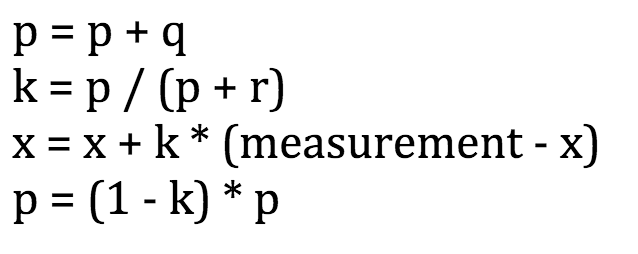
\includegraphics[scale=0.50]{images/kalman.png}
 \caption{Kalman Filter Equations}
 \label{fig:kalman}
\end{figure}

\subsection{Roll and Pitch Measurement}
Using the accelerometer data it is possible to calculate the roll and pitch angle of the board with constant sensitivity using the following equations, where A\textsubscript{x1}, A\textsubscript{y1}, and A\textsubscript{z1} are the acceleration the the x, y and z axis respectively:



\begin{figure}[!htb]
 \centering
 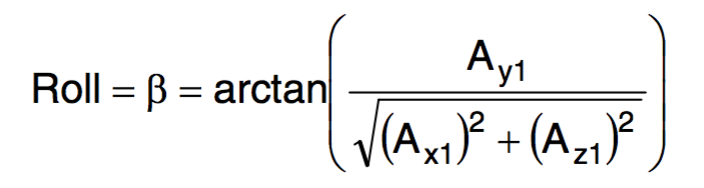
\includegraphics[scale=0.50]{images/roll.png}
 \caption{Measurement of Roll Angle}
 \label{fig:roll}
\end{figure}

\begin{figure}[!htb]
 \centering
 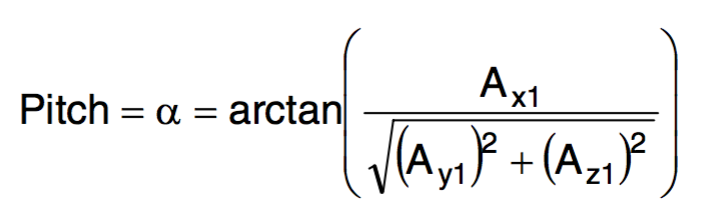
\includegraphics[scale=0.50]{images/pitch.png}
 \caption{Measurement of Pitch Angle}
 \label{fig:pitch}
\end{figure}



\section{Implementation}
\subsection{Accelerometer}
The accelerometer was used with a data rate a 25Hz, a bandwidth of 50Hz, and a full scale of 2g. The accelerometer tell the microcontroller that data is ready by using a pulsed interrupt on the GPIO port E pin 1. The interrupt is set as active high with a priority of 1. After calibrating the sensor, the acceleration data of the x, y and z axis have been filter using the Kalman Filter and then used to measure the roll and pitch angle of the board. \\

The 6 know position measurements were done using the tables in the Lab for z = ±1g. The right angle of the windows in the lab were used to position the board for the measurement of y = ±1 and x = ±1. about 30 measurements were taken in each position an a mean was calculated for each. Then the parameters for the calibration matrix we extracted using equation \ref{cal_eq:2}. The calibration on the raw data was then simply implemented using \ref{cal_eq:1}

\subsection{Threads}

\begin{figure}[!htb]
 \centering
 \includegraphics[scale=0.40]{images/threads.png}
 \caption{Threads Diagram Representation}
 \label{fig:threads}
\end{figure}


\section{Testing and Observations}
\subsection{Thread Visualization}
\subsection{}



\section{Conclusion}

\newpage
\section{Bibliography}
\bibliographystyle{unsrt}
\bibliography{LabReport4} 
\end{document}
